\chapter{Implementación de los Algoritmos Propuestos o  Implementación de ArcGen}\label{cap4}

\section{Herramientas y Lenguajes Utilizados}

\section{Aplicación de Algoritmos: Entorno de Prueba}
Los algoritmos presentados en las secciones \ref{sec:arcdiagram} y \ref{sec:genetico}, tanto el que obtiene un óptimo Crossing Number para grafos completos, como su refinamiento para grafos no completos y finalmente, \textsc{ArcGen}, el algoritmo genético para mejorar el resultado, fueron implementados en lenguaje Java. % y testeados. %A continuación veremos algunos pseudocódigos de estos algoritmos, los cuales utilizan un
	La  representación de Diagrama de Arcos % que se utiliza es la explicada dada en la sección \ref{subsec:representacion_individuos}. 
	%como se mencionó, registra tres arreglos donde
	almacena los nodos, su orden y sus arcos. Los métodos que incluye son: intercambiar nodos, mover un nodo a una posición realizando intercambios, transponer arcos, calcular cruces del grafo y de un arco en particular, calcular grado de arcos y nodos, y nivel de nodo y clonar el grafo.
	
    El algoritmo presentado en la Figura \ref{alg:arcdiagram_trazado}  realiza únicamente el trazado de los arcos como en la Figura \ref{fig:arcdiagram_k6_no_optimo}. Inicialmente,  ordena los nodos por su nivel. En  un grafo completo, el ordenamiento no produce ningún cambio, ya que todos sus nodos tienen el mismo nivel. Sin embargo, en los grafos no completos, permite un ordenamiento inicial más adecuado. Hay que considerar que el algoritmo realiza un recorrido desde el centro hacia los extremos a pesar de que la explicación inicial dada en la sección \ref{sec:arcdiagram} es a la inversa, esto es debido a la manera en que se da la implementación del Diagrama de Arcos y cómo se realizan los inversiones de arcos e intercambios de nodos internamente.
	Por último, el algoritmo invoca al algoritmo para optimizar grafos completos y eliminar los conflictos que genera.
	
	En el algoritmo descripto en la Figura \ref{alg:arcdiagram_optimizado} se presenta la optimización que soluciona los cruces conflictivos para grafos completos y permite obtener el Diagrama de Arcos inicial para lanzar el algoritmo genético.
	
	Finalmente,  se realiza la optimización con el algoritmo genético. El algoritmo presentado en la Figura \ref{alg:genetico} realiza las llamadas a cada ciclo de generaciones hasta encontrar dos ciclos con igual número de cruces o hasta cumplir con $100$ ciclos de tope. Cada ciclo es una llamada al algoritmo de 	generaciones [Figura \ref{alg:genetico_ciclo}], que genera poblaciones,  muta sus individuos, seleccionando los más aptos, \ \ esto es,\ \  aquellos 
		
	\begin{figure}
	    \begin{center}
		\begin{algorithmic}[1]
			\REQUIRE Diagrama de Arcos.
			\STATE Ordenar los nodos según su nivel en orden descendiente.
			\STATE Determina si el número de nodos ($n$) es par o impar.
			\STATE Asigna a un $punteroIzquierdo$ la posición $n/2$.
			\IF {número de nodos par}
			\STATE $punteroDerecho$ comenzará en $n/2 - 1 $.
			\ELSE
			\STATE $punteroDerecho$ comenzará en $n/2 + 1 $.
			\ENDIF
			\STATE Determina el semiplano inicial donde graficar. Si $n$ es par superior sino inferior.
			\FORALL {nodo $\in$ Nodos del grafo}
			\IF {semiplano es superior}
			\STATE Graficar todos los arcos del nodo en $punteroIzquierdo$ en semiplano superior.
			\ELSE 
			\STATE Graficar todos los arcos del nodo en $punteroDerecho$ en semiplano inferior.
			\ENDIF
			\STATE Invierte el semiplano para la próxima iteración.
			\ENDFOR
			\STATE Llamar a algoritmo para optimizar grafo completo con el grafo trazado como entrada.
			\ENSURE Diagrama de Arcos optimizado.
		\end{algorithmic}
	    \end{center}

		\caption{Pseudocódigo para el trazado inicial de un Diagrama de Arcos.}
		\label{alg:arcdiagram_trazado}
	\end{figure}
  
	\begin{figure}
	    \begin{center}
		\begin{algorithmic}[1]
			\REQUIRE Diagrama de Arcos trazado.
			\STATE Calcula el número de transposiciones $t(n) = \floor*{\frac{n}{2}}-2$, con $n > 5$, sino $0$ en caso de $n \leq 5$.
			\STATE Asigna a un $punteroIzquierdo$ la posición 0.
			\STATE Asigna a un $punteroDerecho$ la posición $n-1$.
			\STATE Comienza apuntando al $punteroIzquierdo$.
			\FOR {$i = 0$ hasta $t(n)$}
			\STATE Obtiene los arcos del nodo en el puntero que apunte.
			\STATE Cambia el puntero al opuesto.
			\STATE Inicializa $intercambios$ en $t(n)-i$.
			\WHILE {$j < $ arcos del nodo \AND $intercambios > 0$}
			\STATE Calcula el $CrossingNumber$ actual.
			\STATE Obtiene la $distancia$ entre el nodo actual y el nodo al que conecta el arco.
			\IF {$1 < distancia \leq (t(n)-i+1)$}
			\STATE Invierte el semiplano del arco[$j$].
			\STATE Recalcula el $CrossingNumber$.
			\IF {$CrossingNumber$ es mayor al anterior}
			\STATE Invierte el semiplano del arco[$j$] nuevamente.
			\ENDIF
			\ENDIF
			\ENDWHILE
			\ENDFOR
			\ENSURE Diagrama de Arcos optimizado.
		\end{algorithmic}
	    \end{center}

		\caption{Pseudocódigo para la optimización de Diagrama de Arcos completos.}
		\label{alg:arcdiagram_optimizado}
	\end{figure}
	
	\begin{figure}	
	    \begin{center}
		\begin{algorithmic}[1]
			\REQUIRE Diagrama de Arcos optimizado para completo, un entero $maxCiclos$.
			\STATE Asigna una variable $igualCrossNum$ en falso.
			\WHILE {$i < maxCiclos$ \AND $igualCrossNum$ sea falso}
			\STATE Llamar a algoritmo de ciclo genético y obtener un nuevo grafo.
			\IF {$CrossingNumber$ del grafo anterior es igual al nuevo}
			\STATE Asigna a $igualCrossNum$ verdadero.
			\ENDIF
			\ENDWHILE
			\ENSURE Diagrama de Arcos con optimización genética.
		\end{algorithmic}
	    \end{center}

		\caption{Pseudocódigo para la optimización genética de Diagrama de Arcos no completos.}
		\label{alg:genetico}
	\end{figure}
		\begin{figure}
	    \begin{center}
		\begin{algorithmic}[1]
			\REQUIRE Diagrama de Arcos de ciclo anterior, un entero $maxGeneraciones$.
			\STATE Calcula el $CrossingNumber$ del grafo de entrada, para comparar más adelante.
			\STATE Genera la población inicial con el grafo de entrada.
			\WHILE {$i < maxGeneraciones$ \AND grafo óptimo no encontrado}
			\FORALL {individuo de la población}
			\STATE Muta nodos del individuo con una probabilidad del 30\%.
			\STATE Muta arcos del individuo con una probabilidad del 10\%.
			\IF {individuo es un grafo óptimo (sin cruces)}
			\STATE Corta y devuelve el grafo óptimo.
			\ELSE
			\IF {individuo es peor que el original}
			\STATE Elimina al grafo de la población.
			\ENDIF
			\ENDIF
			\ENDFOR
			\IF {no se encontró grafo óptimo}
			\STATE Ordena los individuos por su fitness (menor CN).
			%\STATE Establece el mejor grafo obtenido de entre los individuos, considerando el mejor de las generaciones anteriores.
			\STATE Obtiene el primer individuo del conjunto (el de mejor fitness).
			% y verifica que tenga mejor fitness que el mejor obtenido en la generación anterior. Si es así lo establece como el mejor, caso contrario permanece el anterior.
			\IF {individuo tiene mejor fitness que mejor individuo de generaciones anteriores}
			\STATE Establece al nuevo individuo como el mejor obtenido.
			\ENDIF
			\ENDIF
			\ENDWHILE
			\ENSURE Diagrama de Arcos óptimo o mejor encontrado.
		\end{algorithmic}
	    \end{center}
		\caption{Pseudocódigo de un ciclo del algoritmo genético.}
		\label{alg:genetico_ciclo}
	\end{figure}
	
	%La generación de población inicial y procesos de mutación  son explicados en la sección \ref{sec:genetico}.
	\begin{figure}
		\centering
		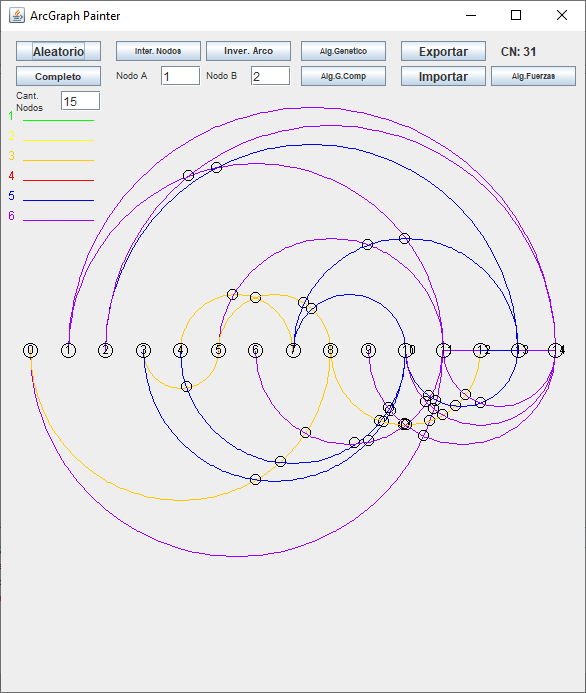
\includegraphics[width=8cm]{imagenes/aplicacion.png}
		\caption{Interfaz de la aplicación desarrollada para visualizar resultados y experimentación.}
		\label{fig:aplicacion}
	\end{figure}
	%Para probar los algoritmos explicados en las secciones anteriores se ha desarrollado una aplicación [Fig. \ref{fig:aplicacion}] que permite la visualización de los Diagrama de Arcos y por otro lado  almacena los resultados de tiempo, ciclos, arcos generados, cruces iniciales y finales de la ejecución del algoritmo genético, siendo que las optimizaciones anteriores son computables rápidamente.

	
	
	
	%\todo[inline,color=green]{COMPLETA}
	
\noindent con menor número de cruces que el grafo semilla y devuelve el mejor grafo obtenido.
	
		En la  Figura \ref{fig:aplicacion}, se muestra la interfaz  de la aplicación desarrollada  que permite la visualización de los Diagramas de Arcos.
		
			Los números en los nodos representan su nombre o identificador,  y permiten diferenciar al nodo sin considerar el 
	 orden en que se disponen en la recta del Diagrama de Arcos.
	
	Los arcos en el gráfico tienen diferentes colores de acuerdo a su Grado de Arco, según la definición dada en la sección \ref{sec:arcdiagram}, con el motivo de visualizar aquellos nodos con más relaciones, según los arcos que conecta.
	
	%\todo[inline,color=green]{COMPLETA idea de  los colores}
	
	%\todo[inline,color=green]{GIULIANO COMPLETA: La aplicación provee una serie de botones con los que se puede generar en forma aleatoria un grafo seteando  parámetros como  ..... los numeros de ExplicarInvertN,  InvertC}
	
	También se dispone de una serie de botones que brindan varias funcionalidades. Los botones \texttt{Random} y \texttt{Complete} permiten generar grafos aleatorio o completos, respectivamente, dada la cantidad de nodos que se especifican en una de las ventanas de texto. 
	
	Los botones \texttt{InvertN} y \texttt{InvertC} permiten invertir el orden de los nodos y transponer un arco dado entre dos nodos, respectivamente, obteniendo los identificadores de los nodos desde las ventanas de texto más pequeñas. 
	
	
	El botón \texttt{Genetic} permite lanzar el algoritmo genético \textsc{\textsc{ArcGen}} sobre el layout del grafo que se está visualizando actualmente, y lo reemplaza finalmente, por el layout resultante. Asimismo,  almacena los resultados de tiempo, ciclos, arcos generados, cruces iniciales y finales de la ejecución del algoritmo genético.
	
	Los botones \texttt{Export} e \texttt{Import} permiten exportar e importar un Diagrama de Arcos, utilizando un formato XML con una estructura propia de la aplicación.
	
	En la parte inferior encontramos los valores \texttt{Population}, \texttt{E.Time} y \texttt{E.Cycles} que indican el tamaño de la población, el tiempo y la cantidad de ciclos, estimados según los registros guardados para el algoritmo genético.	
	%\todo[inline]{almacena o  solo muestra???}
	
	%\todo[inline,color=softred]{R: los almacena, cada vez que se ejecuta el genetico guarda los datos de tiempo, ciclos, etc, y actualiza los valores que muestra en la aplicacion (que son promedios de los guardados).}
	%, siendo que las optimizaciones anteriores son computables rápidamente.
	
	La aplicación está  desarrollada bajo licencia libre y puede accederse a la versión más reciente de su ejecutable a través del repositorio de BitBucket  \url{https://bitbucket.org/giuliano-marinelli/graphlayout}.

\section{Integración con Algoritmo Dirigido por Fuerzas de Tunkelang}